\documentclass[tikz,border=3pt]{standalone}
\usepackage[utf8]{inputenc}
\usepackage[T1]{fontenc}
\usepackage{lmodern}
\renewcommand{\familydefault}{\sfdefault}
\usepackage{sansmath}\sansmath
\usepackage{chemfig}
\usepackage{pgfplots}\pgfplotsset{compat=1.18,/pgf/number format/use comma,/pgf/number format/1000 sep={.}}
\usetikzlibrary{arrows.meta,calc,positioning,decorations.pathmorphing,patterns}
% paleta del sitio
\definecolor{nar}{HTML}{E8680C}\definecolor{narc}{HTML}{FFB35C}\definecolor{hielo}{HTML}{FFF3E8}
\definecolor{tinta}{HTML}{1D1D1F}\definecolor{gris}{HTML}{6E6E73}\definecolor{lila}{HTML}{7C5CF0}
\definecolor{azul}{HTML}{2F6FD6}\definecolor{menta}{HTML}{17A673}\definecolor{coral}{HTML}{E8342A}
\begin{document}
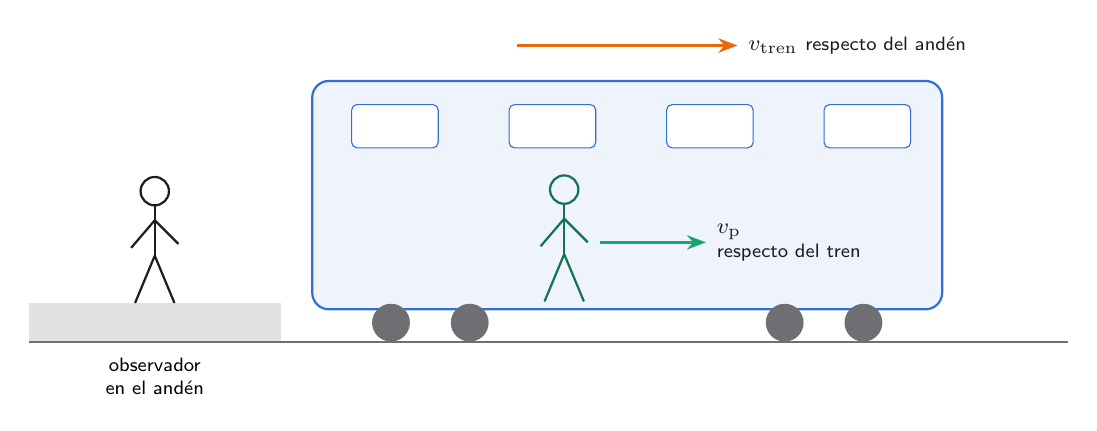
\begin{tikzpicture}[font=\footnotesize,>={Stealth[length=2.4mm]},]

\fill[gris!20] (-3.6,-0.72) rectangle (-0.4,-0.22);
\draw[thick,gris] (-3.6,-0.72) -- (9.6,-0.72);
\draw[thick,azul,fill=azul!8,rounded corners=6pt] (0,-0.3) rectangle (8,2.6);
\foreach \x in {0.5,2.5,4.5,6.5} \draw[azul,fill=white,rounded corners=2pt] (\x,1.75) rectangle (\x+1.1,2.3);
\foreach \x in {1,2,6,7} \fill[gris] (\x,-0.47) circle (0.24);
\draw[menta!70!black,thick] (3.2,1.22) circle (0.18);
\draw[menta!70!black,thick] (3.2,1.04) -- (3.2,0.39999999999999997);
\draw[menta!70!black,thick] (3.2,0.39999999999999997) -- (2.95,-0.2) (3.2,0.39999999999999997) -- (3.45,-0.2);
\draw[menta!70!black,thick] (3.2,0.8500000000000001) -- (2.9000000000000004,0.49999999999999994) (3.2,0.8500000000000001) -- (3.5,0.55);
\draw[->,very thick,menta] (3.65,0.55) -- (5.0,0.55) node[right,align=left,text=tinta] {$v_{\mathrm{p}}$\\[-1pt]{\scriptsize respecto del tren}};
\draw[->,very thick,nar] (2.6,3.05) -- (5.4,3.05) node[right,text=tinta] {$v_{\mathrm{tren}}$ {\scriptsize respecto del andén}};
\draw[tinta,thick] (-2.0,1.2) circle (0.18);
\draw[tinta,thick] (-2.0,1.02) -- (-2.0,0.38);
\draw[tinta,thick] (-2.0,0.38) -- (-2.25,-0.22) (-2.0,0.38) -- (-1.75,-0.22);
\draw[tinta,thick] (-2.0,0.8300000000000001) -- (-2.3,0.48) (-2.0,0.8300000000000001) -- (-1.7,0.53);
\node[font=\scriptsize,align=center] at (-2.0,-1.15) {observador\\en el andén};
\end{tikzpicture}
\end{document}
